\documentclass[12pt,a4paper,oneside]{report}
\usepackage{fontspec}\setmainfont{Times New Roman}
\IfFontExistsTF{Consolas}{\setmonofont{Consolas}}{\setmonofont{Courier New}[Scale=0.85]}
\usepackage[left=3cm,right=2cm,top=2.5cm,bottom=2.5cm,headheight=15pt]{geometry}
\usepackage{amsmath,amssymb,graphicx,longtable,booktabs,array,calc,etoolbox,fancyvrb,fvextra,caption,unicode-math}
\usepackage{needspace,fancyhdr,float}\usepackage[section]{placeins}
\newcounter{none}
\usepackage{xcolor}\definecolor{LinkBlue}{HTML}{1565C0}\usepackage[unicode,colorlinks=true,urlcolor=LinkBlue,linkcolor=black,citecolor=black]{hyperref}\usepackage{xurl,setspace}\onehalfspacing
\hypersetup{hypertexnames=false}
\setlength{\emergencystretch}{3em}\setlength{\parindent}{1cm}
\setlength{\parskip}{3pt}\setlength{\textfloatsep}{16pt}\setlength{\intextsep}{14pt}
\providecommand{\tightlist}{\setlength{\itemsep}{0pt}\setlength{\parskip}{0pt}}
\providecommand{\pandocbounded}[1]{#1}
\renewcommand{\contentsname}{Mục lục}\renewcommand{\chaptername}{Chương}
\renewcommand{\tablename}{Bảng}\renewcommand{\figurename}{Hình}
\renewcommand{\bibname}{Tài liệu tham khảo}\renewcommand{\appendixname}{Phụ lục}\renewcommand{\partname}{Phần}
\renewcommand{\listfigurename}{Danh mục hình}\renewcommand{\listtablename}{Danh mục bảng}
\setcounter{secnumdepth}{2}\setcounter{tocdepth}{2}
\captionsetup{font=small,labelfont=bf,skip=8pt,justification=centering}
\pagestyle{fancy}\fancyhf{}\fancyhead[L]{\small Phát triển các hệ thống thông minh}\fancyhead[R]{\small B23DCCN254}\fancyfoot[C]{\thepage}
\renewcommand{\headrulewidth}{0.3pt}\renewcommand{\footrulewidth}{0pt}
\fancypagestyle{plain}{\fancyhf{}\fancyfoot[C]{\thepage}\renewcommand{\headrulewidth}{0pt}}
\makeatletter
\renewcommand{\thepart}{\Roman{part}.}
\renewcommand*\l@part[2]{\addpenalty{-\@highpenalty}\vskip 1em\begingroup\renewcommand*\numberline[1]{\hb@xt@\@tempdima{##1\hfil}}\bfseries\@dottedtocline{-1}{0em}{1.65em}{#1}{#2}\endgroup}
\renewcommand*\l@chapter[2]{\addpenalty{-\@highpenalty}\vskip .6em\begingroup\bfseries\@dottedtocline{0}{0em}{1.65em}{#1}{#2}\endgroup}
\renewcommand*\l@section{\@dottedtocline{1}{1.65em}{2.45em}}
\renewcommand*\l@subsection{\@dottedtocline{2}{4.1em}{3.15em}}
\renewcommand*\numberline[1]{\hb@xt@\@tempdima{#1.\hfil}}
\renewcommand\@seccntformat[1]{\csname the#1\endcsname.\hspace{.55em}}
\renewcommand\@makechapterhead[1]{\vspace*{10pt}{\parindent\z@\centering\normalfont\ifnum\c@secnumdepth>\m@ne\large\bfseries\@chapapp\space\thechapter\par\nobreak\vskip 10pt\fi\LARGE\bfseries #1\par\nobreak\vskip 25pt}}
\renewcommand\@makeschapterhead[1]{\vspace*{10pt}{\parindent\z@\centering\normalfont\LARGE\bfseries #1\par\nobreak\vskip 25pt}}
\pretocmd{\chapter}{\clearpage}{}{}\pretocmd{\part}{\clearpage}{}{}
\def\@part[#1]#2{%
  \ifnum\c@secnumdepth>-2\relax
    \refstepcounter{part}%
    \addcontentsline{toc}{part}{\protect\numberline{\thepart}#1}%
  \else\addcontentsline{toc}{part}{#1}\fi
  \markboth{}{}%
  {\centering\interlinepenalty\@M\normalfont
    \ifnum\c@secnumdepth>-2\relax\huge\bfseries\partname\nobreakspace\thepart\par\vskip20pt\fi
    \Huge\bfseries#2\par}%
  \@endpart}
\makeatother
\newcommand{\productlink}[2]{\par\medskip\noindent\begin{minipage}{\linewidth}\hrule\vspace{7pt}\textbf{#1}\par\small\url{#2}\par\vspace{7pt}\hrule\end{minipage}\medskip}

\makeatletter
\def\input@path{{../}}
\makeatother
\graphicspath{{../}}
\newcolumntype{P}[1]{>{\raggedright\arraybackslash}p{#1}}
\newcommand{\code}[1]{\texttt{\detokenize{#1}}}
\newcommand{\sourcefile}[1]{\par\noindent{\small\textit{Bằng chứng:} \code{#1}.}\par}
\newcommand{\fig}[3]{\begin{figure}[htbp]\centering\includegraphics[width=#2\linewidth]{#1}\caption{#3}\end{figure}\FloatBarrier}
\newcommand{\thesisBibliographyExtension}{%
  \bibitem{architecture-v2} Trần Đình Quế, \emph{Hybrid Multiagent System Architecture for Diabetes Decision Support}, tài liệu kiến trúc giảng viên cung cấp, tháng 11/2026.
  \bibitem{pima-v2} OpenML, Diabetes, dataset ID 37, phiên bản 1. \url{https://www.openml.org/d/37}.
  \bibitem{early-v2} UCI Machine Learning Repository, Early Stage Diabetes Risk Prediction, dataset ID 529, DOI 10.24432/C5VG8H. \url{https://archive.ics.uci.edu/dataset/529/early+stage+diabetes+risk+prediction+dataset}.
  \bibitem{mlp-v2} Scikit-learn, \emph{MLPClassifier}. \url{https://scikit-learn.org/stable/modules/generated/sklearn.neural_network.MLPClassifier.html}.
  \bibitem{neo4j-v2} Neo4j, \emph{Cypher Manual}. \url{https://neo4j.com/docs/cypher-manual/current/}.%
}
\hypersetup{pdftitle={TIỂU LUẬN FINAL V2},pdfauthor={Kiều Trường Giang},pdfsubject={Phát triển các hệ thống thông minh}}
\begin{document}
\begin{titlepage}\centering
{\large HỌC VIỆN CÔNG NGHỆ BƯU CHÍNH VIỄN THÔNG\\KHOA CÔNG NGHỆ THÔNG TIN 1}\vfill
{\LARGE\bfseries TIỂU LUẬN FINAL V2}\par\vspace{1cm}
{\Large\bfseries HỌC MÁY, BIỂU DIỄN TRI THỨC VÀ HỆ ĐA AGENT}\par\vspace{1cm}
{\large PHÁT TRIỂN CÁC HỆ THỐNG THÔNG MINH}\vfill
\begin{tabular}{ll}Giảng viên:&PGS. TS. Trần Đình Quế\\Sinh viên:&Kiều Trường Giang\\Mã sinh viên:&B23DCCN254\\Nhóm học phần:&06\\Nhóm thực hiện:&02\end{tabular}\vfill
Hà Nội, tháng 11 năm 2026
\end{titlepage}
\pagenumbering{roman}
\tableofcontents\clearpage
\listoffigures\clearpage
\listoftables\clearpage
\pagenumbering{arabic}
\chapter*{Mở đầu}\addcontentsline{toc}{chapter}{Mở đầu}
Báo cáo nghiên cứu cách kết hợp học máy, học sâu và biểu diễn tri thức trong một hệ thống hỗ trợ người dùng. Phần I trình bày lịch sử AI, các mô hình học máy trên dữ liệu bảng, CNN trên ảnh và RNN trên chuỗi. Phần II đi từ Knowledge Graph và RAG đến học sâu trên đồ thị, phối hợp đa agent và học tăng cường. Thực nghiệm Cora đối chiếu GCN với MLP, còn mô phỏng Agent02 khảo sát chính sách theo luật và chính sách học tăng cường.

Tiểu luận Final V2 phát triển từ bản Final bằng Phần III. Chương~\ref{ch:v2-protocol} xây dựng hai thực nghiệm tiểu đường có quy trình dữ liệu chung. Chương~\ref{ch:v2-mlp} huấn luyện và phân tích mạng MLP năm tầng ẩn. Chương~\ref{ch:v2-agents} nối mô hình với KB, Neo4j và RAG trong hệ đa agent. Chương~\ref{ch:v2-verification} kiểm tra kết quả, phân tích giới hạn và hướng dẫn tái lập.

Các kết quả trong hai phần đầu thuộc những thực nghiệm của bản Final. Các số liệu của Phần III được ghi theo hai bộ dữ liệu, cấu hình và checkpoint cụ thể. Báo cáo Project 01 trình bày cách triển khai và vận hành ứng dụng GlucoGuide.
\input{abbreviations.tex}
\input{data_overview.tex}
\part{Nền tảng và tổng hợp}
\input{thesis_core.tex}
\input{theory_extension.tex}
\part{Phát triển thực nghiệm và hệ thống V2}
\chapter{Thiết kế thực nghiệm tiểu đường V2}\label{ch:v2-protocol}

\section{Câu hỏi nghiên cứu và liên hệ với bản Final}
Chương 2 khảo sát mô hình học máy trên dữ liệu bảng. Các chương CNN, RNN và GCN minh họa ba loại cấu trúc đầu vào khác. V2 quay lại dữ liệu bảng để khảo sát một câu hỏi có thể kiểm tra trực tiếp. Khi thêm hai tầng ẩn và điều chỉnh quá trình huấn luyện, sai số của MLP thay đổi thế nào trên hai bộ dữ liệu có cách thu thập khác nhau? Phân tích xét cả số mẫu dương tính được nhận diện và số mẫu âm tính bị báo nhầm.

Thực nghiệm gồm Logistic Regression làm đối chứng tuyến tính, MLP ba tầng ẩn theo hình dạng V1 và MLP năm tầng ẩn của V2. Hai MLP được huấn luyện trên cả Pima lẫn Early Stage. V1 đối chứng là kiến trúc được huấn luyện lại theo giao thức của chương này. Mô hình V1 gốc trên bộ 50K và các kết quả đã trình bày trong Phần I giữ vai trò bối cảnh. Mỗi chỉ số mới gắn với một bộ dữ liệu, một phép chia và một cấu hình cụ thể.

\par\FloatBarrier\begin{table}[H]\centering\small\setstretch{1.15}\setlength{\tabcolsep}{5pt}
\caption{V1 và phần nâng cấp V2 có thể kiểm tra.}\begin{tabular}{P{2.6cm}P{5.6cm}P{5.6cm}}\toprule
Hạng mục & V1 gốc / đối chứng & V2\\\midrule
Dữ liệu model & 50K nhãn tổng hợp và hồi quy; giữ nguyên checkpoint gốc. & Thêm Pima và Early Stage nhị phân; kiểm kê trùng và nguồn.\\
Mạng đối chứng & Ba tầng ẩn 64--32--16. & Năm tầng ẩn 64--32--16--8--4, L2 mạnh hơn và trọng số lớp cân bằng.\\
MAS & Có MessageBus và các handler chuyên trách. & Thêm workflow riêng sáu tầng, bảy vai trò, schema theo dataset.\\
Truy vết & Trace sender/receiver/type/content trong response. & Thêm request ID, version, status, timing, hash và audit metadata.\\
KB / KG / chat & 58 đoạn, 169 nút, 106 cạnh, TF-IDF và Qwen4B. & Tái sử dụng nguyên; không nhận là các thành phần mới hoặc fine-tune mới.\\
Tài liệu nộp & Tiểu luận Final, Project 01 và các tệp thực nghiệm. & Tiểu luận phát triển từ Final, Project 01, Cypher, ZIP và hướng dẫn.\\\bottomrule\end{tabular}\end{table}


\section{Nguồn, quần thể và đơn vị quan sát}
Pima lấy từ OpenML 37, phiên bản 1 \cite{pima-v2}. Dữ liệu lịch sử gồm 768 bản ghi, tám đặc trưng đầu vào và nhãn phân loại nhị phân. Mẫu thuộc quần thể nữ từ 21 tuổi. Phạm vi này ảnh hưởng cách hiểu kết quả, kể cả khi chương trình nhận một bộ giá trị có hình thức hợp lệ. Các phép đo glucose, huyết áp, insulin và BMI có đơn vị riêng. Giá trị phả hệ là một chỉ số của bộ dữ liệu.

Early Stage lấy từ UCI 529 \cite{early-v2}. Dữ liệu thu từ bảng hỏi ở Sylhet, Bangladesh, có tuổi, giới tính và 14 trường triệu chứng hoặc đặc điểm. Nhãn gắn với quá trình thu thập của nghiên cứu đó. Các trường Yes/No được chuyển sang 1/0 theo từ điển đầu vào. Mỗi bộ có mô hình, bộ tiền xử lý và hợp đồng nhập liệu riêng. Sự khác nhau về quần thể, loại phép đo và nhãn giới hạn diễn giải khi đặt các chỉ số của hai bộ cạnh nhau.

\par\FloatBarrier\begin{table}[H]\centering\small\setstretch{1.15}\setlength{\tabcolsep}{5pt}
\caption{Hai bộ dữ liệu và phép chia thực tế sau làm sạch.}\begin{tabular}{P{4.2cm}rr}\toprule
Hạng mục & Pima & Early Stage\\\midrule
Nguồn & OpenML 37 v1 & UCI 529\\
Số dòng gốc & 768 & 520\\
Sau loại trùng & 768 & 251\\
Số feature & 8 & 16\\
Train / validation / test & 460 / 154 / 154 & 150 / 50 / 51\\
Negative / Positive (sạch) & 500 / 268 & 78 / 173\\
Nhóm feature mâu thuẫn & 0 & 0\\\bottomrule\end{tabular}\end{table}

\par\FloatBarrier\begin{table}[H]\centering\small\setstretch{1.15}\setlength{\tabcolsep}{5pt}
\caption{Tám feature Pima; đơn vị theo mô tả nguồn, không phải ngưỡng chẩn đoán.}\begin{tabular}{P{2.2cm}P{6.5cm}P{5cm}}\toprule
Mã & Ý nghĩa & Đơn vị / xử lý\\\midrule
preg & Số lần mang thai & Số lần; 0 hợp lệ\\
plas & Plasma glucose sau 2 giờ OGTT & mg/dL; 0 coi là thiếu\\
pres & Huyết áp tâm trương & mmHg; 0 coi là thiếu\\
skin & Nếp gấp da cơ tam đầu & mm; 0 coi là thiếu\\
insu & Insulin huyết thanh sau 2 giờ & $\mu$U/mL; 0 coi là thiếu\\
mass & Chỉ số BMI & kg/m$^2$; 0 coi là thiếu\\
pedi & Diabetes pedigree function & Điểm chỉ số của dataset\\
age & Tuổi & Năm; quần thể từ 21 tuổi\\\bottomrule\end{tabular}\end{table}

\par\FloatBarrier\begin{table}[H]\centering\small\setstretch{1.15}\setlength{\tabcolsep}{5pt}
\caption{Từ điển 16 đặc trưng của Early Stage theo thứ tự mô hình.}\begin{tabular}{P{5.2cm}P{5.3cm}P{4.0cm}}\toprule
Trường gốc & Ý nghĩa & Dạng đầu vào\\\midrule
Age & Tuổi & Tuổi theo năm\\
Gender & Giới tính (nam=1, nữ=0) & 0 = nữ, 1 = nam\\
Polyuria & Tiểu nhiều & 0 = không, 1 = có\\
Polydipsia & Khát nhiều & 0 = không, 1 = có\\
sudden weight loss & Sụt cân đột ngột & 0 = không, 1 = có\\
weakness & Yếu sức & 0 = không, 1 = có\\
Polyphagia & Ăn nhiều & 0 = không, 1 = có\\
Genital thrush & Nấm sinh dục & 0 = không, 1 = có\\
visual blurring & Nhìn mờ & 0 = không, 1 = có\\
Itching & Ngứa & 0 = không, 1 = có\\
Irritability & Dễ cáu & 0 = không, 1 = có\\
delayed healing & Chậm lành vết thương & 0 = không, 1 = có\\
partial paresis & Yếu/liệt một phần & 0 = không, 1 = có\\
muscle stiffness & Cứng cơ & 0 = không, 1 = có\\
Alopecia & Rụng tóc & 0 = không, 1 = có\\
Obesity & Béo phì (mã dataset) & 0 = không, 1 = có\\\bottomrule\end{tabular}\end{table}


\section{Chuẩn hóa bản ghi và chống giao nhau giữa các tập}
Trước khi chia, chương trình lập chữ ký từ vector đặc trưng để nhận diện các bản ghi có cùng đầu vào. Nếu cùng vector có nhãn mâu thuẫn, cả nhóm bị loại. Nếu nhãn giống nhau, giữ bản ghi đầu tiên. Kiểm tra phát hiện 269 dòng trùng ở Early Stage và không phát hiện nhóm mâu thuẫn. Sau bước này, Early Stage còn 251 mẫu. Trên Pima, bước kiểm tra không loại bản ghi. Chữ ký dựa trên dữ liệu quan sát. Một người có thể xuất hiện ở nhiều hàng với giá trị khác nhau vì nguồn thiếu mã người tham gia.

Ở Pima, giá trị 0 trong năm trường đo gồm glucose, huyết áp, độ dày nếp da, insulin và BMI được biểu diễn thành thiếu. Số lần mang thai bằng 0 là giá trị hợp lệ. Quy tắc này áp dụng trước phép chia. Trung vị để điền thiếu và thống kê chuẩn hóa được học sau khi chia, chỉ từ tập train. Phép biến đổi trên validation và test dùng lại cùng tham số. Nếu một trường có trung bình \(\mu_j\) và độ lệch chuẩn \(\sigma_j\) học trên train, giá trị sau điền thiếu được biến đổi theo
\[
    z_{ij}=\frac{x_{ij}-\mu_j}{\sigma_j}.
\]
Pipeline đóng gói thứ tự điền thiếu, chuẩn hóa và suy luận. Khi các trường được gửi theo thứ tự khác, Data Agent ghép chúng theo tên trong registry trước khi đưa vào pipeline.

\par\FloatBarrier\begin{table}[H]\centering\small\setstretch{1.15}\setlength{\tabcolsep}{5pt}
\caption{Phân bố nhãn theo từng tập sau khi làm sạch.}\begin{tabular}{llrrr}\toprule
Bộ dữ liệu & Tập & Negative & Positive & Tổng\\\midrule
Pima & train & 299 & 161 & 460\\
Pima & validation & 100 & 54 & 154\\
Pima & test & 101 & 53 & 154\\
Early Stage & train & 47 & 103 & 150\\
Early Stage & validation & 15 & 35 & 50\\
Early Stage & test & 16 & 35 & 51\\\bottomrule\end{tabular}\end{table}


\section{Vai trò của train, validation và test}
Mỗi bộ được chia xấp xỉ 60/20/20 theo lớp bằng seed chia 254. Train dùng để fit tiền xử lý và trọng số. Validation chọn epoch. Test mô tả kết quả sau khi checkpoint được chọn. Trên mỗi bộ, Logistic, V1 và V2 dùng chung các hàng và cùng tiền xử lý. Điều kiện này cho phép đối chiếu các mô hình ở cấp từng bản ghi.

Ba seed 254, 255, 256 kiểm tra độ nhạy với khởi tạo và xáo minibatch. Chúng dùng chung phép chia, vì vậy trung bình và độ lệch chuẩn mô tả biến thiên giữa các lần tối ưu trên đúng dữ liệu đó. Seed 254 được dùng cho demo để có một checkpoint xác định trước. Tập test đã được dùng trong các lần thực nghiệm V2 trước đó, nên kết quả ở đây mang tính so sánh trên bộ dữ liệu đã biết. Một tập mới độc lập sẽ hữu ích để xác nhận.

\section{Vai trò của đối chứng tuyến tính}
Logistic Regression học một tổ hợp tuyến tính trước sigmoid. Nó cho biết một đường phân tách đơn giản hoạt động ra sao trên phép chia hiện tại. Hai MLP có khả năng học tổ hợp phi tuyến. V2 thay đổi đồng thời độ sâu, L2 và trọng số lớp. Muốn định lượng riêng ảnh hưởng của độ sâu, cần huấn luyện các cấu hình trung gian với cùng L2 và trọng số lớp rồi lặp lại qua nhiều phép chia.

\sourcefile{data/v2/sources/sources.json}
\sourcefile{scripts/train_v2.py}
\sourcefile{results/v2/experiment.json}

\chapter{Mạng năm tầng ẩn và phân tích kết quả}\label{ch:v2-mlp}

\section{Cấu trúc lớp và phép tính tiến}
Mỗi tầng ẩn áp dụng một phép biến đổi affine, sau đó dùng ReLU. Với \(a^{(0)}=x\) và \(\ell=1,\ldots,5\), ta có
\[
    z^{(\ell)}=W^{(\ell)}a^{(\ell-1)}+b^{(\ell)},\qquad
    a^{(\ell)}=\max(0,z^{(\ell)}).
\]
Sigmoid biến giá trị ở đầu ra thành điểm \(p\) trong khoảng 0 đến 1. Ở ngưỡng 0,5, hệ thống gán nhãn Positive khi \(p\geq0{,}5\). Ý nghĩa của nhãn do từng bộ dữ liệu quy định. Phần giữa đầu vào và đầu ra có đúng năm tầng, lần lượt 64, 32, 16, 8 và 4 neuron. Cấu hình V1 đi từ 64 qua 32 đến 16 neuron, rồi sang đầu ra.

\fig{figures/mlp.png}{0.95}{Năm tầng ẩn của V2. Đầu vào có tám hoặc 16 đặc trưng tùy bộ dữ liệu.}

Hai tầng bổ sung 8 và 4 neuron nén dần biểu diễn trước khi tính điểm. Mạng Pima có 3.361 tham số, tính theo công thức \(\sum_\ell(n_{\ell-1}+1)n_\ell\):
\[
  (8+1)64+(64+1)32+(32+1)16+(16+1)8+(8+1)4+(4+1)1=3361.
\]
Early Stage thêm tám đầu vào vào tầng 64 neuron, làm số tham số tăng \(8\times64=512\) so với Pima. Vì vậy mạng có 3.873 tham số. V1 có 3.201 và 3.713 tham số tương ứng. Thay đoạn kết 16--1 của V1 bằng đoạn 16--8--4--1 làm tổng số tham số tăng 160 trên mỗi bộ. Phép đếm bao gồm bias và có thể kiểm tra từ kích thước ma trận trong checkpoint.

\section{Mục tiêu tối ưu và chọn checkpoint}
Hàm mất mát nhị phân phạt dự đoán sai mạnh hơn khi mô hình gán điểm với độ tự tin cao. Với trọng số mẫu \(w_i\), phần dữ liệu của hàm mất mát có dạng
\[
 -\frac{1}{\sum_i w_i}\sum_i w_i
 \big[y_i\log p_i+(1-y_i)\log(1-p_i)\big].
\]
V1 dùng trọng số mẫu bằng nhau và hệ số L2 \(10^{-4}\). V2 dùng trọng số cân bằng \(w_c=N/(2N_c)\), tính riêng từ số mẫu lớp \(c\) trên train, cùng hệ số L2 \(10^{-2}\). Như vậy lớp ít mẫu được tăng đóng góp tương đối vào hàm mất mát. L2 làm giảm khuynh hướng tăng độ lớn trọng số. Với Early Stage, lớp thiểu số là Negative. Với Pima, lớp thiểu số là Positive. Điều này giúp giải thích vì sao cân bằng lớp có thể thay đổi kiểu sai số khác nhau giữa hai bộ.

Adam dùng learning rate \(10^{-3}\), batch tối đa 32 và tối đa 600 epoch \cite{mlp-v2}. Sau mỗi epoch, mô hình tính macro-F1 validation ở ngưỡng 0,5. Nếu bằng điểm, chọn epoch có log loss validation thấp hơn. Dừng nếu qua 60 epoch liên tiếp chưa cải thiện tiêu chí. Checkpoint là bản sao tại epoch tốt nhất. Mô hình dùng chính trọng số này để dự đoán test. Việc fit lại trên cả train và validation sẽ sinh một checkpoint khác.

\par\FloatBarrier\begin{table}[H]\centering\small\setstretch{1.15}\setlength{\tabcolsep}{5pt}
\caption{Epoch được chọn theo validation và macro-F1 trên test theo từng seed.}\begin{tabular}{llrrrr}\toprule
Bộ dữ liệu & Model & Seed & Epoch & F1 validation & F1 test\\\midrule
Pima & V1 & 254 & 16 & 0.7703 & 0.7267\\
Pima & V1 & 255 & 33 & 0.7779 & 0.7351\\
Pima & V1 & 256 & 13 & 0.7550 & 0.7471\\
Pima & V2 & 254 & 5 & 0.7780 & 0.7210\\
Pima & V2 & 255 & 24 & 0.7772 & 0.7150\\
Pima & V2 & 256 & 72 & 0.7710 & 0.6587\\
Early Stage & V1 & 254 & 10 & 0.9048 & 0.8145\\
Early Stage & V1 & 255 & 5 & 0.8571 & 0.7935\\
Early Stage & V1 & 256 & 17 & 0.8417 & 0.9015\\
Early Stage & V2 & 254 & 46 & 0.9271 & 0.8741\\
Early Stage & V2 & 255 & 24 & 0.8498 & 0.9348\\
Early Stage & V2 & 256 & 18 & 0.9048 & 0.9015\\\bottomrule\end{tabular}\end{table}

\fig{figures/learning.png}{0.96}{Log loss validation theo epoch trên hai bộ dữ liệu, seed 254. Tiêu chí chọn đầu tiên là macro-F1 validation.}

Trên Pima seed 254, V1 chọn epoch 16 và V2 chọn epoch 5. Trên Early Stage, V1 chọn epoch 10 và V2 chọn epoch 46. Độ sâu vì thế không quyết định một số epoch chung cho mọi bộ. Log loss và macro-F1 có thể đạt điểm tốt nhất ở các epoch khác nhau vì log loss xét độ lớn điểm dự đoán, còn F1 dựa trên nhãn sau ngưỡng.

\section{Đọc chỉ số theo từng bộ dữ liệu}
Accuracy là tỷ lệ dự đoán đúng. Recall Positive bằng \(TP/(TP+FN)\) và precision Positive bằng \(TP/(TP+FP)\). F1 là trung bình điều hòa của precision và recall. Macro-F1 lấy trung bình F1 của hai lớp. Ví dụ, trên Pima seed 254, V2 có \(TP=40\), \(FN=13\), \(FP=28\). Recall Positive đạt \(40/53\approx0{,}755\) và precision Positive đạt \(40/68\approx0{,}588\).

\par\FloatBarrier\begin{table}[H]\centering\small\setstretch{1.15}\setlength{\tabcolsep}{5pt}
\caption{Metric test; trung bình $\pm$ độ lệch chuẩn khởi tạo, không phải khoảng tin cậy.}\begin{tabular}{llrrrl}\toprule
Dataset & Mạng & Accuracy & Macro-F1 & Recall + & Tham số\\\midrule
Pima & Logistic & 0.773 & 0.734 & 0.566 & --\\
Pima & V1 & 0.762 $\pm$ 0.008 & 0.736 $\pm$ 0.008 & 0.654 $\pm$ 0.009 & 3201\\
Pima & V2 & 0.712 $\pm$ 0.026 & 0.698 $\pm$ 0.028 & 0.723 $\pm$ 0.044 & 3361\\
Early Stage & Logistic & 0.980 & 0.977 & 1.000 & --\\
Early Stage & V1 & 0.876 $\pm$ 0.033 & 0.837 $\pm$ 0.047 & 0.990 $\pm$ 0.013 & 3713\\
Early Stage & V2 & 0.922 $\pm$ 0.016 & 0.903 $\pm$ 0.025 & 0.971 $\pm$ 0.040 & 3873\\\bottomrule\end{tabular}\end{table}

\fig{figures/two_datasets.png}{0.96}{Macro-F1 test theo từng bộ dữ liệu. Vạch sai số là độ lệch chuẩn ba lần khởi tạo. Logistic có một lần chạy.}
\par\FloatBarrier\begin{table}[H]\centering\small\setstretch{1.15}\setlength{\tabcolsep}{5pt}
\caption{Ma trận nhầm lẫn ở seed demo 254; lớp Positive là lớp 1.}\begin{tabular}{llrrrr}\toprule
Dataset & Mạng & TN & FP & FN & TP\\\midrule
Pima & V1 & 82 & 19 & 19 & 34\\
Pima & V2 & 73 & 28 & 13 & 40\\
Early Stage & V1 & 9 & 7 & 0 & 35\\
Early Stage & V2 & 11 & 5 & 0 & 35\\\bottomrule\end{tabular}\end{table}

Ở seed demo 254, Pima có accuracy V1/V2 là 0.7532/0.7338, macro-F1 0.7267/0.7210, recall Positive 0.6415/0.7547. Chênh lệch accuracy ghép cặp V2 trừ V1 là -0.0195, khoảng bootstrap 95\% [-0.0779, 0.0325]. Logistic đối chứng đạt macro-F1 0.7336.

Ở seed demo 254, Early Stage có accuracy V1/V2 là 0.8627/0.9020, macro-F1 0.8145/0.8741, recall Positive 1.0000/1.0000. Chênh lệch accuracy ghép cặp V2 trừ V1 là 0.0392, khoảng bootstrap 95\% [0.0000, 0.0980]. Logistic đối chứng đạt macro-F1 0.9768.

Trung bình ba seed, V2 tăng macro-F1 trên Early Stage. Trên Pima, recall Positive tăng và macro-F1 giảm. Hai khoảng bootstrap đều chứa 0. Độ sâu, L2 và trọng số lớp thay đổi cùng lúc. Hai tập test đã được dùng trước đó. Cần dữ liệu mới để xác nhận.


Trên Pima, số mẫu dương tính bị bỏ sót ở seed demo giảm từ 19 còn 13 khi chuyển sang V2. Số báo dương tính nhầm tăng từ 19 lên 28. Tổng dự đoán đúng giảm ba bản ghi, tương đương 1,95 điểm phần trăm accuracy. Trung bình qua ba seed, recall Positive tăng từ 0,654 lên 0,723, trong khi macro-F1 giảm từ 0,736 xuống 0,698.

Trên Early Stage, ở seed demo cả hai cấu hình nhận ra 35 mẫu Positive. V2 dự đoán đúng thêm hai mẫu Negative, nên accuracy tăng 3,92 điểm phần trăm trên 51 mẫu. Trung bình ba seed, macro-F1 của V2 đạt 0,903 so với 0,837 của V1. Logistic đạt 0,977 trên phép chia này. Kết quả của Logistic cho thấy mô hình đơn giản vẫn là một đối chứng quan trọng với dữ liệu có ít đặc trưng và ít mẫu.

\subsection{Theo dõi mẫu đổi trạng thái giữa hai mô hình}
\par\FloatBarrier\begin{table}[H]\centering\small\setstretch{1.15}\setlength{\tabcolsep}{5pt}
\caption{Thay đổi dự đoán trên cùng hàng test, seed 254, thứ tự V1 tới V2.}\begin{tabular}{llrrrrr}\toprule
Bộ dữ liệu & Nhãn thật & Đúng/đúng & Đúng/sai & Sai/đúng & Sai/sai & Tổng\\\midrule
Pima & Negative & 72 & 10 & 1 & 18 & 101\\
Pima & Positive & 33 & 1 & 7 & 12 & 53\\
Early Stage & Negative & 9 & 0 & 2 & 5 & 16\\
Early Stage & Positive & 35 & 0 & 0 & 0 & 35\\\bottomrule\end{tabular}\end{table}

Hai ma trận nhầm lẫn cho biết tổng số lỗi của từng mô hình. Để tìm mẫu đã đổi kết quả, ghép điểm V1 và V2 theo chỉ số hàng test. Ví dụ trên 53 mẫu Positive của Pima, 33 mẫu được cả hai dự đoán đúng, một mẫu chuyển từ đúng sang sai, bảy mẫu chuyển từ sai sang đúng, 12 mẫu sai ở cả hai. Bảy lượt sửa và một lỗi mới tạo mức tăng ròng sáu mẫu dương tính đúng. Trong lớp Negative, một lượt sửa và mười lỗi mới làm số mẫu âm tính đúng giảm chín. Chênh lệch accuracy trên toàn bộ Pima bằng \((6-9)/154\). Trên Early Stage seed 254, cả hai thay đổi có lợi đều ở lớp Negative.

So sánh ghép cặp giữ cùng đầu vào và nhãn, cho phép xem mức thay đổi theo từng lớp. Nó cũng là dữ liệu đầu vào cho khoảng bootstrap ở mục sau. Phân tích theo từng hàng giúp lý giải vì sao recall Positive của V2 có thể cao hơn khi accuracy và macro-F1 thấp hơn trên Pima.

\section{Khoảng bất định và giới hạn suy diễn}
Để so sánh accuracy theo cặp, đặt \(d_i=\mathbf{1}[\hat{y}_{i,V2}=y_i]-\mathbf{1}[\hat{y}_{i,V1}=y_i]\). Chênh lệch quan sát là trung bình \(d_i\). Bootstrap lấy lại các chỉ số hàng test có hoàn lại 2.000 lần và lấy percentile 2,5\% và 97,5\%. Giữ cặp theo hàng giúp hai dự đoán luôn được đánh giá trên cùng bản ghi. Hai khoảng đều chứa 0, trong đó cận dưới Early Stage bằng 0.

Một phép chia và ba seed khởi tạo chưa đo được mức thay đổi qua cơ sở thu thập, quần thể hoặc thời gian. Các chỉ số phản ánh bài toán phân loại nhãn của bộ dữ liệu. Nghiên cứu tiếp theo có thể dùng nhiều phép chia theo nhóm, khóa bộ test mới và khảo sát độ hiệu chuẩn bằng tập validation riêng. Thí nghiệm tách thành phần cần thay một yếu tố mỗi lượt, giữ các yếu tố còn lại cố định và theo dõi cả thời gian học lẫn sai số theo lớp.

\chapter{Tích hợp mô hình với KB, Neo4j và RAG}\label{ch:v2-agents}

\section{Hai đường dữ liệu hội tụ ở điều phối}
Các chương trước trình bày mô hình học dựa trên ví dụ và kho tri thức dựa trên tài liệu. Trong GlucoGuide, nhánh mô hình nhận một vector đặc trưng để trả điểm và nhãn nghiên cứu. Nhánh tri thức nhận câu hỏi để lấy đoạn nguồn và cạnh đồ thị. Coordinator tổ chức thứ tự chạy. Explanation trình bày hai loại kết quả trong cùng phản hồi. Đường huấn luyện mô hình dùng Pima và Early Stage. Đường xây KB dùng tài liệu web và PDF có vị trí đối chiếu.

\fig{figures/provenance.png}{0.92}{Đường đi của dữ liệu huấn luyện và tài liệu tri thức trong V2.}

\section{Sáu tầng và bảy vai trò}
Kiến trúc theo tài liệu giảng viên \cite{architecture-v2} được áp dụng trong một backend local. Giao diện hiển thị biểu mẫu và kết quả. Tầng API kiểm tra yêu cầu theo hợp đồng từng bộ dữ liệu. Tầng điều phối chọn thứ tự gọi các tác vụ. Tầng agent chuyên trách xử lý dữ liệu, mô hình, luật, tri thức, giải thích và nhật ký. Tầng tri thức và mô hình chứa các tài nguyên thực thi. Tầng đánh giá cung cấp kết quả kiểm thử, số đo và dấu vết.

\par\FloatBarrier\begin{table}[H]\centering\small\setstretch{1.15}\setlength{\tabcolsep}{5pt}
\caption{Bảy vai trò: Coordinator điều phối sáu agent chuyên trách.}\begin{tabular}{P{2.2cm}P{4.1cm}P{4.1cm}P{3.1cm}}\toprule
Vai trò & Đầu vào & Đầu ra & Thực hiện\\\midrule
Coordinator & Request + dataset/version & Response tích hợp hoặc lỗi & Workflow trong v2.py\\
Data & Feature thô và schema & Feature order, missing flags hoặc lỗi & validate\_data\\
Prediction & Dữ liệu chuẩn hóa & Label, score, threshold, version, hash & predict / pipeline\\
Rule & Dataset, cờ dữ liệu & Cờ phạm vi và giới hạn & reviewed\_rules\\
KG/RAG & Câu hỏi kiến thức & Đoạn có nguồn, cạnh đã đối chiếu & Retriever + GraphKnowledgeAgent\\
Explanation & Model + rules + evidence & Giải thích có nguồn, không chẩn đoán & explain\\
Monitoring & Metadata lượt chạy & Trạng thái lưu request/version & monitor / JSONL\\\bottomrule\end{tabular}\end{table}

\fig{figures/layers.png}{0.70}{Sáu tầng tổ chức phần mềm. Coordinator điều phối sáu vai trò chuyên trách.}

Một lần thực nghiệm bắt đầu bằng việc cấp mã yêu cầu. Data Agent kiểm tra tập tên trường, giá trị hữu hạn và các miền đã khai báo. Prediction Agent dùng đúng checkpoint của phiên bản được chọn. Rule Agent nhận dữ liệu và dự đoán, đối chiếu tính nhất quán của điểm, ngưỡng, nhãn và gắn cờ phạm vi. Kết quả bất nhất bị chặn trước Explanation. KG/RAG Agent truy xuất đoạn và đối chiếu cạnh. Explanation Agent kết hợp điểm nghiên cứu và thông tin nguồn. Monitoring Agent lưu metadata. API trả trace gắn mã yêu cầu để người xem nhận ra mỗi bước được gọi và kết thúc thế nào.

Khi yêu cầu chứa tình huống ưu tiên, bước an toàn chặn việc gọi mô hình. Dữ liệu sai hợp đồng dừng ở bước kiểm tra. Nếu Neo4j gián đoạn, phản hồi ghi trạng thái đồ thị và có thể dùng bằng chứng văn bản từ KB. Các tình huống này được kiểm tra riêng để người xem nhận biết nguồn thông tin đang có.

\section{Nguồn tri thức, chỉ mục và truy vấn cạnh}
KB hợp nhất \textbf{58 đoạn từ 22 nguồn đang được sử dụng}, gồm \textbf{21 link web và 1 PDF}. Mỗi nguồn được ít nhất một đoạn tham chiếu. Mục \code{sources} trong \href{https://github.com/jellalaz/He_Thong_Thong_Minh_Thay_Que/blob/main/exports/KB_KG_RAG/KB_knowledge.json}{KB\_knowledge.json trên GitHub} liệt kê đủ 22 URL. Nhóm có đối chiếu trích đoạn trong \nolinkurl{data/source_curation.json} gồm ba bài web (một NIDDK và hai Vinmec) cùng một PDF NIDDK \emph{Guiding Principles}, đóng góp 12 đoạn.

Bản xuất KG gồm 169 nút \code{Concept} và 106 cạnh \code{RELATED_TO}. Thuộc tính document nối quan hệ về đoạn KB, evidence lưu đoạn làm căn cứ và source URL chỉ tới nguồn. Tệp \code{kb_diabet.cypher} nằm trong \nolinkurl{exports/KB_KG_RAG/}. Mã nguồn và dữ liệu thực nghiệm có tại \href{https://github.com/jellalaz/He_Thong_Thong_Minh_Thay_Que}{repo GlucoGuide trên GitHub}.

\par\FloatBarrier\begin{table}[H]\centering\small\setstretch{1.15}\setlength{\tabcolsep}{5pt}
\caption{Năm bộ ba thật từ KB đang nạp, kèm mã tài liệu đối chiếu.}\begin{tabular}{P{3.4cm}P{3.2cm}P{3.7cm}P{3cm}}\toprule
Chủ thể & Quan hệ & Đối tượng & Document\\\midrule
HbA1c & phản ánh & đường huyết trung bình & \code{a1c}\\
Glucose & cần có & đơn vị và thời điểm đo & \code{testing}\\
Tiểu đường & liên quan đến & thiếu hoặc sử dụng insulin kém hiệu quả & \code{overview}\\
Vận động & hỗ trợ & quản lý đường huyết & \code{activity}\\
Liều thuốc & cần được chỉ định bởi & nhân viên y tế & \code{medicine}\\\bottomrule\end{tabular}\end{table}


RAG biểu diễn văn bản bằng TF-IDF từ và ký tự. Chế độ xếp hạng áp ngưỡng và giữ tối đa bốn đoạn. Một số chủ đề dùng danh sách nguồn đã định tuyến. KG Agent lấy tối đa bốn mã tài liệu và đối chiếu cạnh với đoạn gốc. Với truy vấn trong Neo4j \cite{neo4j-v2}, điều kiện \code{r.document = 'a1c'} lấy các cạnh ứng với nguồn HbA1c. Kết quả có thể đối chiếu với bản xuất JSON và chi tiết nguồn ở giao diện.

\begin{Verbatim}[fontsize=\small,breaklines=true]
MATCH (a:Concept)-[r:RELATED_TO]->(b:Concept)
WHERE r.document = 'a1c'
RETURN a.name, r.label, b.name, r.evidence, r.source_url
\end{Verbatim}

Nhánh trò chuyện dùng Qwen3 4B local để sinh câu trả lời từ ngữ cảnh. Nhánh thực nghiệm MLP dùng mẫu giải thích có nguồn. Mac chạy Neo4j trực tiếp và lưu audit tệp. Vercel có thể dùng bản chụp đồ thị khi Aura gián đoạn. Hai nhánh dùng chung kho tri thức và có cách tạo đầu ra riêng. Checkpoint V2 lưu mô hình phân loại dạng bảng. Trọng số Qwen thuộc mô hình trò chuyện.

\section{Một ví dụ có dấu vết thực thi}
Với mẫu công khai của Pima, câu hỏi HbA1c được đưa vào nhánh tri thức. Cùng mẫu đó cho điểm Positive 0,5239 ở V1 và 0,5472 ở V2 trong lượt kiểm thử đã lưu. Hai điểm cùng nằm trên ngưỡng 0,5 nên nhãn giữ nguyên. Bước KG/RAG chọn mã tài liệu \code{a1c}, đối chiếu hai cạnh và trả nguồn. Lượt chạy có 12 thông điệp, gồm yêu cầu và kết quả cho sáu vai trò chuyên trách.

Để kiểm tra tại lớp, mở mục Thực nghiệm V1/V2, điền mẫu công khai, chọn V2 và chạy. Màn hình cho thấy năm kích thước lớp. Mở trace để đọc model version và mã yêu cầu. Sau đó đổi V1 đối chứng trên cùng mẫu để so số lớp và điểm. Nguồn \code{a1c} minh họa đường đi của tri thức. Trong Neo4j Browser, tìm cạnh theo mã nguồn và kiểm tra trường evidence. Ví dụ thể hiện khả năng truy vết hệ thống. Nhận xét về chất lượng mô hình dựa trên toàn bộ tập test.

Project 01 V2 mở rộng ví dụ này thành ba bằng chứng: cặp ảnh dự đoán cùng mẫu Pima, đồ thị con của mã \code{a1c} và một lượt Trò chuyện dùng Qwen với nguồn \code{plate}. Các ảnh giúp phân biệt đầu ra mô hình phân loại, căn cứ từ Neo4j và văn bản sinh ở ba bước triển khai.

\begin{figure}[htbp]
\centering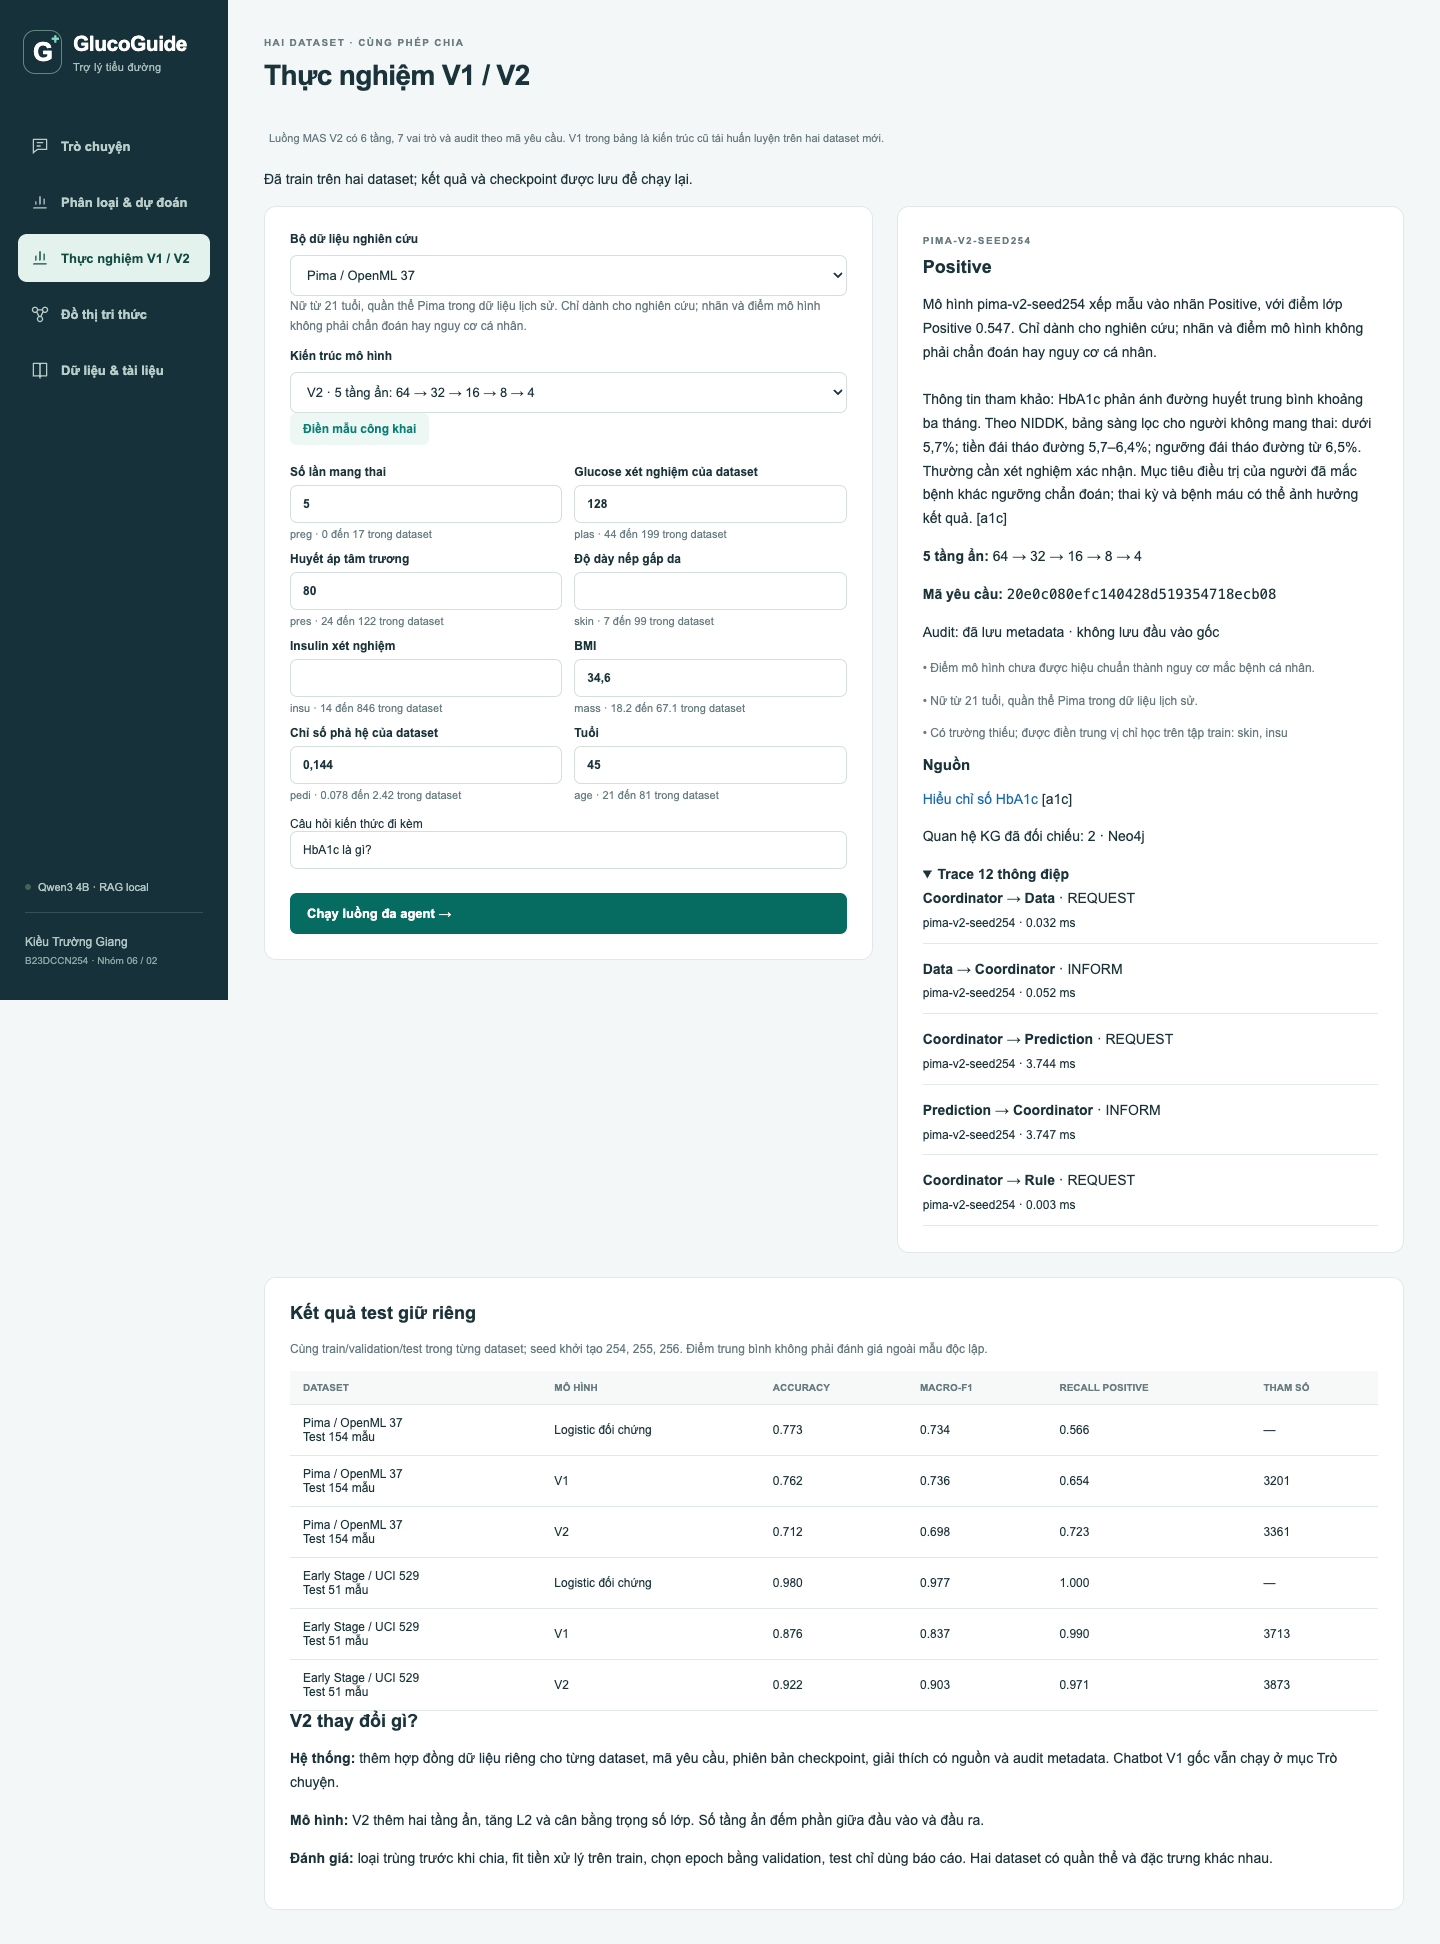
\includegraphics[width=\linewidth,height=0.55\textheight,keepaspectratio]{figures/demo-v2.png}
\caption{Demo V2 trên Mac với mô hình năm tầng, kết quả, nguồn và dấu vết thực thi.}
\end{figure}
\FloatBarrier

\chapter{Kiểm chứng, tái lập và phát triển tiếp}\label{ch:v2-verification}

\section{Đối chiếu từ số liệu trong báo cáo tới tệp gốc}
Kết quả huấn luyện nằm trong \code{results/v2/experiment.json}. Tệp ghi cấu hình, seed, epoch tốt nhất, chỉ số và mã băm checkpoint demo. Hai CSV test lưu chỉ số hàng, nhãn thực và điểm của từng cấu hình qua ba seed. Có thể chọn cột \code{v2_254_prob}, áp ngưỡng 0,5 và đếm lại bốn ô của ma trận. Tệp \code{learning_curves.csv} lưu lịch sử train loss, log loss validation và macro-F1 validation theo từng epoch.

Mô hình demo gồm tiền xử lý và MLP trong cùng tệp \code{.joblib}. Registry ghi tên trường và phạm vi của từng bộ. Khi load pipeline và chạy lại các hàng trong CSV test, kết quả phải khớp với điểm đã lưu tới sai số tuyệt đối \(10^{-12}\). Phép thử kiểm tra liên kết giữa model triển khai và số liệu báo cáo. Mã băm SHA-256 xác định phiên bản tệp. Khi huấn luyện lại, cần lưu cấu hình và số liệu của chính lần chạy mới.

\par\FloatBarrier\begin{table}[H]\centering\small\setstretch{1.15}\setlength{\tabcolsep}{5pt}
\caption{Đối chiếu từng loại bằng chứng với vị trí trong gói mã nguồn.}\begin{tabular}{P{4.4cm}P{5.2cm}P{4.7cm}}\toprule
Bằng chứng & Vị trí & Cách kiểm tra\\\midrule
Nguồn và hợp đồng dữ liệu & \code{data/v2/sources/} & Xem nguồn, phiên bản và dữ liệu gốc.\\
Phép chia train, validation, test & \code{data/v2/pima.csv} và \code{early_stage.csv} & Đếm nhãn, hàng và khóa đặc trưng theo tập.\\
Điểm từng hàng test & \code{results/v2/} & Dùng cột xác suất và ngưỡng 0,5 để lập lại ma trận.\\
Checkpoint và registry & \code{models/v2/} & Đối chiếu thứ tự đặc trưng và SHA-256.\\
Vết chạy đa agent & \code{results/v2/} và \code{agent_examples.json} & Xem model version, mã yêu cầu và mã đoạn nguồn.\\
Kho tri thức và chỉ mục & \code{exports/diabetes/} & Đọc KB, Cypher và phát lại bộ câu truy xuất.\\\bottomrule\end{tabular}\end{table}


\section{Kiểm chứng hệ thống và khả năng chạy lại}
Bộ kiểm thử V2 chạy bốn tổ hợp giữa hai bộ dữ liệu và hai phiên bản trên API. Nó kiểm tra phân chia dữ liệu, điểm dự đoán, hình dạng lớp, nguồn, cạnh đồ thị, dấu vết và nhật ký. Các ca lỗi dùng trường thiếu, giá trị không hữu hạn, yêu cầu ưu tiên và tình huống graph gián đoạn. Kiểm thử giao diện trên Mac chạy cùng luồng và xác nhận danh sách phiên bản hiển thị đúng cấu hình. Kiểm thử truy xuất offline phát lại 22 câu từ bộ xuất để kiểm tra chỉ mục và kết quả truy xuất.

\par\FloatBarrier\begin{table}[H]\centering\small\setstretch{1.15}\setlength{\tabcolsep}{5pt}
\caption{Bằng chứng kiểm thử thực tế; kiểm thử phần mềm không là chứng nhận lâm sàng.}\begin{tabular}{P{5.4cm}P{8.5cm}}\toprule
Nhóm & Kết quả / nơi kiểm tra\\\midrule
V2 tích hợp & 13 kiểm tra qua; results/v2/integration\_checks.json.\\
Model parity & Hai dataset, hai version seed 254: xác suất khớp CSV test tới sai số 1e-12.\\
Graph coverage & 58/58 tài liệu, 106 cạnh; exact triples, evidence và URL khớp KB.\\
Export & 8 nhóm; checksum, CSV và thư mục phẳng, replay 22 câu offline, Cypher EXPLAIN.\\
V1 regression suite & Nguồn/PDF, an toàn, feedback, intent, graph, model support và UI trên Mac.\\
Live chat & 13 lượt smoke test local; 7 lượt sinh Qwen kèm context KG; không là benchmark y khoa.\\\bottomrule\end{tabular}\end{table}


Tại thư mục gốc, chạy \code{bash run-macos.sh start} để bật Neo4j, mô hình ngôn ngữ local và web. Dùng \code{.venv/bin/python -m scripts.train_v2} để huấn luyện lại hai mô hình nghiên cứu từ dữ liệu đã lưu. Khi demo, dùng checkpoint trong gói. Dữ liệu và kết quả của bản Final có đường tái lập riêng, gồm mã Cora trong phụ lục và các artifact được dẫn tại từng chương.

\section{Giới hạn của dữ liệu, mô hình và truy xuất}
Hai bộ dữ liệu có kích thước nhỏ và quần thể khác nhau. Kết quả chỉ có thể so trực tiếp giữa các cấu hình trong cùng bộ. Kiến trúc, L2 và trọng số lớp thay đổi đồng thời nên cần kiểm tra từng yếu tố riêng để giải thích nguyên nhân. Kết quả Qwen có nguồn vẫn cần kiểm tra nội dung khi mở rộng phạm vi câu hỏi. Hit@K đo sự hiện diện của nguồn trong danh sách truy xuất. Để đánh giá nội dung sinh ra, cần đối chiếu từng khẳng định với nguồn và xem hệ thống xử lý câu hỏi thiếu căn cứ ra sao.

\subsection{Đối chiếu đại lượng đo trong từng lớp hệ thống}
Kết quả phân loại được đối chiếu ở cấp hàng test. Kết quả truy xuất được đối chiếu ở cấp mã đoạn, với Hit@1, Hit@4 và MRR@4. Ma trận nhầm lẫn kiểm tra lỗi của nhãn dự đoán, còn các chỉ số truy xuất kiểm tra vị trí của nguồn kỳ vọng. Đầu ra bằng văn bản cần thêm đánh giá câu trả lời theo từng mệnh đề. Ở cấp hệ thống, yêu cầu 422, bypass an toàn và fallback Neo4j kiểm tra các nhánh khác nhau của điều phối. Các phép đo có mẫu số và mục tiêu riêng.

Ở tầng audit, mã yêu cầu liên kết với phiên bản và hash model. Trace trả về cho demo cho thấy thông điệp, còn tệp nhật ký chỉ lưu metadata cần để kiểm tra lượt chạy. Thời gian điều phối tới trước bước lưu được tách với thời gian phản hồi end-to-end tại trình duyệt. Khi làm benchmark cần ghi điều kiện máy, trạng thái warm-up, số lượt và phân vị độ trễ cho từng nhánh.

\section{Hướng phát triển theo câu hỏi kiểm chứng}
\begin{enumerate}
\item \textbf{Độ bền của mô hình.} Khóa tập test mới và dùng nhiều phép chia theo nhóm khi có mã người tham gia. Báo cáo chỉ số theo từng lớp, quy mô của mỗi nhóm và độ bất định qua các phép chia.
\item \textbf{Giá trị của độ sâu.} So sánh ba và năm tầng dưới cùng hệ số L2, cùng trọng số lớp và cùng bộ dữ liệu. Sau đó thay riêng L2 hoặc trọng số lớp. Ghi cả thời gian học và sai số theo lớp.
\item \textbf{Khả năng truy xuất.} Bổ sung câu hỏi diễn đạt lại và ghi nhãn nguồn phù hợp trước khi chạy. Đánh giá việc tìm đúng đoạn, dùng đúng đoạn và xử lý câu không có nguồn đủ rõ.
\item \textbf{Chi phí điều phối.} Đo thời gian từng tác vụ và tỷ lệ trường hợp lấy được căn cứ hợp lệ khi Neo4j hoặc bộ sinh gián đoạn. Ghi các phép đo theo mã yêu cầu và phiên bản model.
\end{enumerate}

\input{thesis_conclusion.tex}
\section*{Kết quả bổ sung của V2}
Hai thực nghiệm V2 cho thấy thay đổi kiến trúc cần được đọc cùng đặc điểm của dữ liệu và ma trận nhầm lẫn. Mạng năm tầng ẩn cải thiện macro-F1 trên Early Stage trong phép chia đã dùng. Trên Pima, recall dương tính tăng và macro-F1 giảm. Các kết quả này gợi ý kiểm tra thêm qua nhiều phép chia, tách riêng ảnh hưởng của độ sâu, L2 và trọng số lớp, rồi xác nhận bằng dữ liệu mới.

Ở cấp hệ thống, GlucoGuide V2 đưa thông tin phiên bản mô hình, nguồn truy xuất và kết quả từng bước vào cùng một lượt chạy. Tệp Cypher, chỉ mục RAG, dữ liệu test, checkpoint và nhật ký kỹ thuật tạo thành đường đối chiếu từ báo cáo đến demo.
\input{bibliography_thesis.tex}
\appendix
\chapter{Mã nguồn tái lập}
\section{scripts/train\_cora.py}
\VerbatimInput[fontsize=\scriptsize,breaklines=true,breakanywhere=true]{../../scripts/train_cora.py}
\chapter{Mã nguồn chính của V2 có chú thích}\label{ch:v2-core-code}

Các đoạn dưới được lấy trực tiếp từ mã nguồn của bộ nộp. Số ở lề trái là số dòng trong tệp gốc. Phần chữ trước và sau mỗi đoạn giải thích dữ liệu vào, tác dụng của lệnh và kết quả chuyển sang bước tiếp theo. Các tệp đầy đủ nằm trong repository.

\newcommand{\vTwoExcerpt}[3]{%
  \par\noindent\textit{\nolinkurl{#1}, dòng #2--#3.}\par
  \VerbatimInput[fontsize=\small,breaklines=true,breakanywhere=true,numbers=left,
    numbersep=5pt,xleftmargin=1.5em,firstline=#2,lastline=#3,firstnumber=#2]{../../#1}%
}

\section{Đọc dữ liệu và khóa phép chia}
Cấu hình V1/V2 nằm ở dòng 35--38. Hai tuple mô tả số neuron ở các tầng giữa. \code{alpha} đặt mức L2 và \code{balanced} bật trọng số lớp trong V2.
\vTwoExcerpt{scripts/train_v2.py}{35}{38}

\code{load_data} chuyển nhãn nguồn thành 0/1, xử lý 0 ở các trường đo của Pima và chuẩn hóa các mã của Early Stage. Phần chữ ký nhận diện vector trùng trước khi tạo tập test. Nếu các bản ghi cùng vector có nhãn khác nhau, cả nhóm bị loại khỏi bộ sạch.
\vTwoExcerpt{scripts/train_v2.py}{59}{79}

Hai lần \code{train_test_split} tạo train và phần còn lại, rồi chia phần còn lại thành validation và test. Dòng 108--109 fit pipeline trên train và chỉ transform ở hai tập sau. Nhờ đó giá trị trên validation và test không tham gia tính trung vị hoặc scaler.
\vTwoExcerpt{scripts/train_v2.py}{97}{111}

\section{Huấn luyện, chọn epoch và lưu checkpoint}
Dòng 118--121 tạo model và trọng số mẫu. \code{partial_fit} học trên train. Điểm dùng để chọn checkpoint lấy từ validation. Bộ \code{score} ưu tiên macro-F1 cao, rồi log loss thấp. \code{deepcopy} giữ bản sao tại epoch được chọn, vì mô hình còn được cập nhật ở các epoch sau. Sau vòng học, dòng 132 mới dự đoán test. Seed 254 lưu mô hình cùng imputer và scaler, nên dịch vụ gọi được cả pipeline từ một tệp.
\vTwoExcerpt{scripts/train_v2.py}{118}{143}

\section{Kiểm đầu vào và suy luận một mẫu}
Data Agent lấy tên trường có thứ tự từ registry. Nó phân biệt giá trị thiếu với khóa thiếu, kiểm số hữu hạn và mã nhị phân. Trong Pima, quy tắc 0 thành thiếu giống quy tắc khi chuẩn bị dữ liệu. Đầu ra trả danh sách tên, giá trị theo thứ tự và các trường thiếu để Prediction dùng đúng cột.
\vTwoExcerpt{app/v2.py}{63}{87}

\code{predict} dựng DataFrame một hàng rồi gọi \code{predict_proba}. Dòng 94 chọn cột lớp 1 theo \code{classes_}. Kết quả có điểm, nhãn theo ngưỡng 0,5, số tầng, phiên bản và hash. Rule Agent nhận dự đoán và dữ liệu, kiểm tra điểm, ngưỡng và nhãn, rồi gắn cờ phạm vi.
\vTwoExcerpt{app/v2.py}{90}{115}

\section{Điều phối và gộp kết quả}
Đoạn đầu tạo mã lượt và kiểm an toàn trước Prediction. Nếu Data Agent báo lỗi, Coordinator trả 422 và ghi metadata nhánh lỗi. Khi hợp lệ, nó gọi Prediction, Rule và KG/RAG. Dòng 172--177 kiểm tra và chặn kết quả không nhất quán. Dòng 187 đưa cả ba kết quả cho Explanation. Dòng 189--196 ghi metadata và trả nguồn, cạnh và trace về web.
\vTwoExcerpt{app/v2.py}{153}{196}

\section{Truy xuất văn bản và đối chiếu Neo4j}
Retriever xử lý ba đường vào: bỏ qua truy xuất, nguồn đã được chỉ định, hoặc xếp hạng. Với xếp hạng, điểm từ và ký tự được gộp, bổ sung điểm cụm từ và điểm định tuyến, rồi áp ngưỡng để chọn kết quả.
\vTwoExcerpt{app/retrieval.py}{47}{76}

Neo4j nhận mã tài liệu dưới dạng tham số. Dòng 17--29 kiểm tra bộ ba, đoạn trích và URL so với KB. Truy vấn lưu trong hằng \code{FACT_QUERY}; phần dữ liệu đầu vào được truyền riêng khi gọi driver. Kết quả hợp lệ mới được chuyển sang khâu giải thích.
\vTwoExcerpt{app/graph_knowledge.py}{4}{8}
\vTwoExcerpt{app/graph_knowledge.py}{15}{29}
\vTwoExcerpt{app/graph_knowledge.py}{46}{53}

\section{Tạo ngữ cảnh cho Qwen và bảo vệ phản hồi}
Trong luồng Trò chuyện, prompt ghép đoạn và cạnh đã đối chiếu. \code{respond} chọn phản hồi bảo vệ nếu có cờ hoặc thiếu căn cứ. Khi gọi Qwen local, nó gửi bản nháp cho verifier và có thể sinh lại một lần. Sau đó trả văn bản đã qua kiểm hoặc phương án KB.
\vTwoExcerpt{app/local_prompt.py}{18}{27}
\vTwoExcerpt{app/local_llm.py}{41}{57}

\ifdefined\projectCodeAppendix
\section{Nối giao diện, backend và dịch vụ local}
Giao diện biến giá trị trống thành \code{null}, gửi dataset và version tới API, rồi đọc phản hồi JSON. Script chạy local chờ Neo4j, nạp graph, bật Qwen qua llama.cpp và khởi động web. Các dòng dưới giúp đối chiếu thứ tự với trạng thái demo.
\vTwoExcerpt{web/v2.js}{10}{15}
\vTwoExcerpt{scripts/local_stack.py}{96}{114}

\section{Kiểm thử đối chiếu checkpoint và trace}
Test đọc các hàng test đã lưu, tính lại xác suất qua pipeline và yêu cầu khớp tới sai số \(10^{-12}\). Sau đó gọi API với mẫu công khai và kiểm số tầng, nguồn, graph và tập vai trò. Một phép thử gắn bảng kết quả với model, phép thử kia gắn model với đường demo.
\vTwoExcerpt{scripts/test_v2.py}{28}{42}
\fi

\end{document}
